\DiaryEntry{FIR Filter Design}{2016-09-29}{Optimization}

\subsection{Problem Definition}

We want to design a linear phase filter. The filter order \(n = 2N+1\)
is odd and the impulse response is symmetric around the midpoint:

\[
h_k = H_{n-k-1}, \quad k=0,\ldots,n-1
\]

We therefore have \(h_0 = h_{n-1}, h_1 = h_{n-2} \ldots\). The
corresponding frequency response \(H(e^{j \omega}\) depends only on
\(h_0,\ldots,h_N\) and is given by

\[
H(e^{j \omega} = h_0 + h_1 e^{j\omega} + h_2 e^{j2\omega} + \cdots h_{n-1} e^{j(n-1)\omega} = e^{-jN\omega} \left( 2h_0 \cos N \omega  + 2 h_1 (N-1) \omega + \cdots + h_N \right) = e^{-jN} \tilde{H}(e^{j \omega})
\]

This shows that the filter has a linear phase; the absolute value of the
frequency response is given by \(\tilde{H}(e^{j\omega})\).

In order to obtain an optimization problem, we discretize the problem;
i.e.~we calculate \(\tilde{H}(e^{j\omega})\) at a discrete number of
points. We can then write the expression for this discretized frequency
response as

\[
\mathbf{\tilde{H}} = \mathbf{W} \mathbf{h}
\]

where the i-th row of \(\mathbf{W}\) contains the values
\([\cos(\omega_i N), \cos(\omega_i (N-1)), \ldots,1]\) and
\(\mathbf{h}\) is a column vector containing the \(N\) filter
coefficients.

\subsection{Optimization Problem}

We can now define our filter design problem such that we defne a
passband and a stopband and we seek a filter with maximal stopband
attenuation, while having a defined ripple in the passband.


\begin{align*}
\min & |\mathbf{W}_s h| \\
s.t. & \mathbf{W}_p h > \delta_1 \\
     & \mathbf{W}_p h < \delta_2 \\
\end{align*}


Here, \(\mathbf{W}_s\) and \(\mathbf{W}_p\) denote the rows of
\(\mathbf{W}\) corresponding to frequencies in the passband and
stopband, respectively, and \(\delta_1, \delta_2\) denotes the ripple in
the passband.

\subsection{Solution via CvxPy}

The following script defines and solves the optimization problem above

\begin{verbatim}
# Number of FIR coefficients (including the zeroth one).
n = 20
# passfreq.
wpass = 1.2
# passripple
pass_max = 1.1
pass_min = 0.9
# stopfreq.
wstop = 1.6

# Rule-of-thumb frequency discretization (Cheney's Approx. Theory book).
m = 15*n
w = np.mat(np.linspace(0,np.pi,m)).T
# the i-th row of A contains the values [2cos w_i N 2cos w_1 (N-1) ... 1]
A = np.cos(  np.kron(np.mat(w), np.mat(np.arange(n-1,-1,-1)))  )
# indices for splitting the frequency matrix
ind_pass = np.where(w < wpass)
ind_stop = np.where(w > wstop)
# the splitted matrices
Apass = A[ind_pass[0], :]
Astop = A[ind_stop[0], :]

# definition of optimization problem
h = cvx.Variable(n)
# objective function -> mas stopband attenuation
obj = cvx.Minimize( cvx.sum_squares( Astop * h))
# passband ripple as constraint
con = [Apass * h > pass_min, Apass * h < pass_max]

# Solve problem.
prob = cvx.Problem(obj, con)
prob.solve()

print("status:", prob.status)
print("optimal value", prob.value)
print("optimal var", h.value)

# calc. frequency response
H = A * h.value
Hpass = Apass*h.value

# and plot it...
plt.plot(w, 20*np.log10(np.abs(H)))
plt.xlabel(r'$\omega$')
plt.ylabel(r'$|H(\omega)|$ in dB')
plt.title('FIR filter freq. response magnitude')

plt.grid()
\end{verbatim}

\subsection{Example}

Using the following values: n = 20, wpass =1.2, wstop = 1.6, pass\_max =
1.1, pass\_min = 0.9 we obtainth efollowing plot of the frequency
response:

\begin{figure}[H]
\centering
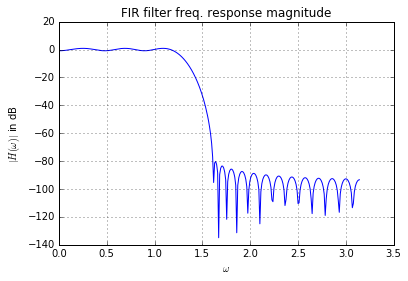
\includegraphics{images/fir_design_1.png}
\end{figure}

If we decrease the gap between passband and stopband (wpass =1.5, wstop
= 1.6) and leave all other parameters unchanged, the stopband
attenuation decreases as is shown below. In other words, a sharper
filter provides less stoppband attenuation.

\begin{figure}[H]
\centering
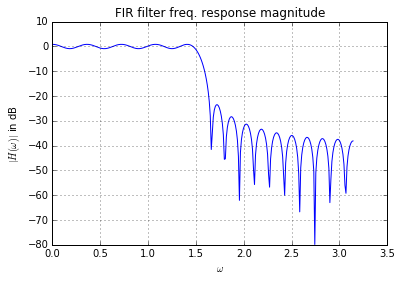
\includegraphics{images/fir_design_2.png}
\end{figure}

If we allow more filter coefficients (in this case n = 80), then we
achieve a higher stoppband attenuation as below (even though the filter
is sharper).

\begin{figure}[H]
\centering
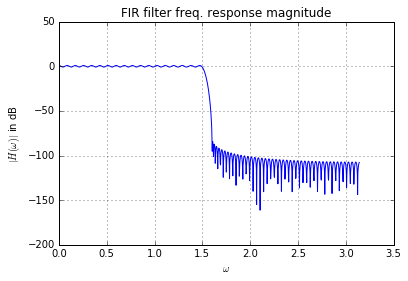
\includegraphics{images/fir_design_3.png}
\end{figure}
